The spread of COVID-19 has elevated the importance of epidemiological
models as a means to forecast both near- and long-term spread. 
In the United States, the Institute for Health Metrics and Evaluation (IHME)
model has emerged as a key influencer of state- and national-level
policy \citep{covid2020forecasting}.  
The IHME model includes a detailed characterization
of the variation in
hospital bed capacity, ICU beds, and ventilators between and within
states. Predicting the projected strains on underlying
health resources is critical to supporting planning efforts.
However such projections require
an epidemic `forecast'.  The IHME's epidemic forecast
differs from conventional
epidemic models in a significant way -- IHME assumes
that the cumulative deaths in the COVID-19 epidemic 
follow a symmetric, Gaussian-like trajectory. 
For example, the 
IHME model predicts that if the peak is 2 weeks away then in 4 weeks
cases will return to the level of the present, and continue
to diminish rapidly.  But, epidemics need not have one symmetric peak -- 
the archaic Farr's Law of Epidemics notwithstanding
(see~\citep{bregman1990farr} for a cautionary tale of using
Farr's law as applied to the HIV epidemic). 

Conventional epidemic
models represent populations in terms of their `status' vis
a vis the infectious agent, in this case 
SARS-CoV-2 (e.g.,~\citep{ferguson2020report,kucharski2020early,kissler_medrxiv2020,park_medrxiv2020,kraemer_2020sci,li_science2020,wu2020estimating}), e.g.,
susceptible, exposed, infectious,
hospitalized, and recovered.  
New transmission can lead to an exponential increases in cases 
when the basic reproduction number ${\cal{R}}_0>1$ (the
basic reproduction number denotes the average number of new
infections caused by a single, typical individual in an otherwise
susceptible population \citep{anderson1991infectious}).  Subsequent
spread, if left unchecked, would yield a single peak -- in theory. That 
peak corresponds to when `herd immunity' is reached, such
that the effective reproduction number, $\Reff=1$.
The effective reproduction number denotes the number of new
infectious cases caused by a single infectious individual
in a population with pre-existing circulation.
But, even when herd immunity is reached, there will still be new cases 
which then diminish over time, until the epidemic concludes.  
A single-peak paradigm is
only robust insofar as the disease has spread
sufficiently in a population to reach and exceed `herd immunity'.
The converse
is also true in the case of COVID-19 -- as long as 
a population remains predominantly immunologically
naive, then the risk of further infection has not passed. 

The Imperial College of London (ICL) model~\citep{ferguson2020report} is
one of the most influential of 
epidemiogical models shaping public health responses to COVID-19. The ICL model is an
example of a `conventional' epidemic model
that shows the benefits of  early intervention steps in reducing
transmission and preserving health system resources vs.~a `herd immunity' strategy.  
The ICL model assumes that
transmission is reduced because of externalities, like lockdowns,
school closings, and so on.  
As a result, the ICL model suggests that lifting of large-scale
public health interventions could be followed by a second wave of cases.
Yet, for a disease
that is already the documented cause of more than 50,000 deaths
in the United States, we posit that individuals
are likely to continue to modify
their behavior even after lockdowns are lifted.  
Hence, here, we use a simple model to
ask the question: what is the anticipated
shape of an epidemic if individuals modify their behavior in direct
response to the impact of a disease at the population level? In doing so,
we build upon earlier work on awareness based models (e.g.~\citep{funk2009spread,funk2010modelling,eksin2017disease, eksin2019systematic}) with a
simple, initial assumption: individuals reduce interactions when 
death rates are high and increase interactions when death rates are low.  

To begin, consider a SEIR like model
\begin{eqnarray}
\dot{S} &=& -\frac{\beta SI}{\left[1+\left(\delta/\delta_c\right)^{k}\right]}\\
\dot{E} &=& \frac{\beta SI}{\left[1+\left(\delta/\delta_c\right)^{k}\right]}-\mu E\\
\dot{I} &=& \mu E-\gamma I \\
\dot{R} &=& (1-f_D)\gamma I\\
\dot{D} &=& f_D\gamma I
\end{eqnarray}
%\begin{eqnarray}
%\dot{S} &=& -\beta SI a(\vec{x}) \\
%\dot{E} &=& \beta SI} a(\vec{x})}-\mu E\\
%\dot{I} &=& \mu E-\gamma I \\
%\dot{R} &=& (1-f_D)\gamma I
%\dot{D} &=& f_D)\gamma I
%\end{eqnarray}
%where $a(\vec{x})$ denotes awareness-based distancing given the
%epidemiological phase space
where $S$, $E$, $I$, $R$, and $D$ denote the proportions of
susceptible, exposed, infectious, recovered, and deaths, respectively.
The awareness-based distancing is controlled by 
the death rate $\delta\equiv \dot{D}$,
the half-saturation constant ($\delta_c>0$), and
the sharpness of change in the force of infection ($k\geq 1$).
Since $\delta$ is proportional to $I$, this model is closely related to a recently proposed awareness-based distancing model~\citep{eksin2019systematic}.
Note that the present
model converges to the conventional SEIR model as $\delta_c\rightarrow \infty$.
\begin{figure}[t!]
\begin{center}
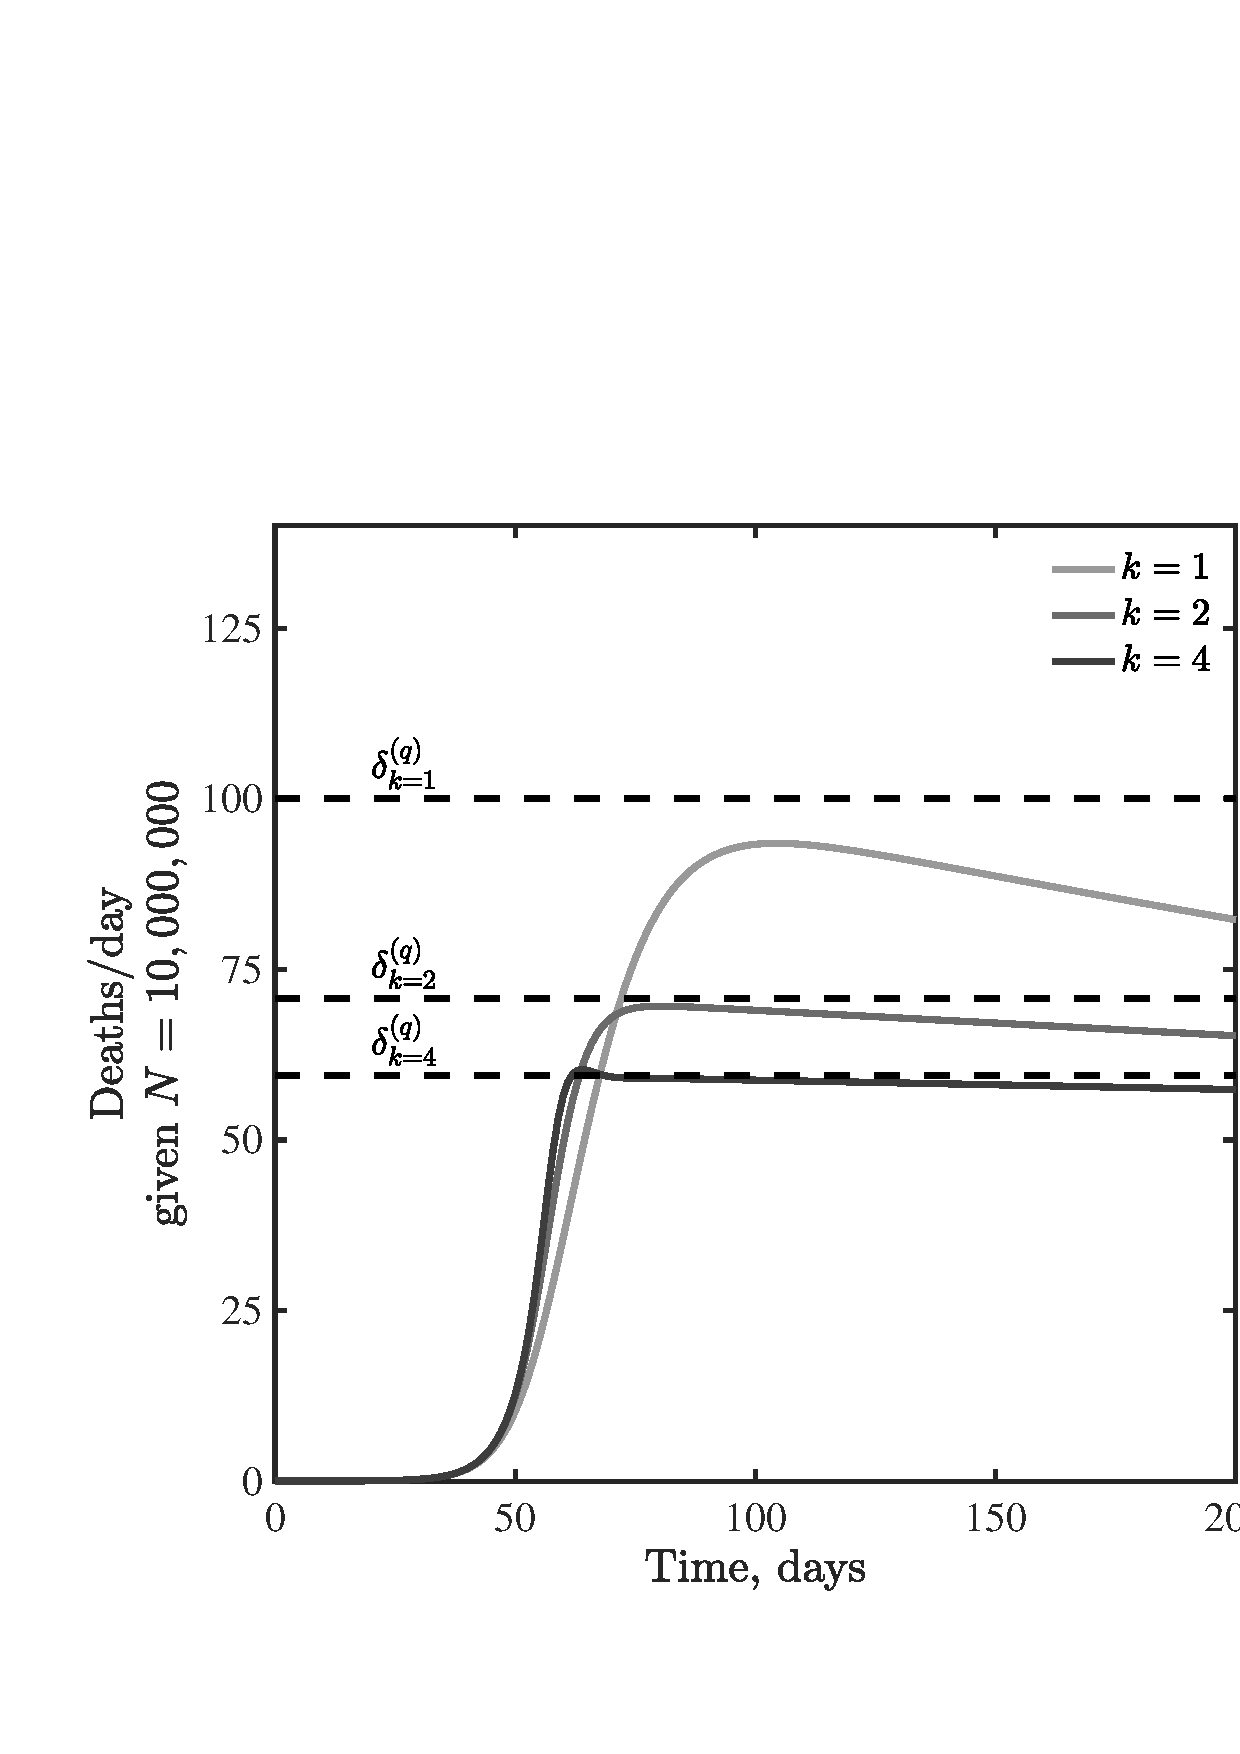
\includegraphics[width=0.4\textwidth]{scripts/figseir_baseplat_k2_D_noname.pdf}\\
\includegraphics[width=0.4\textwidth]{scripts/figseir_baseplat_k2_I_noname.pdf}
\caption{Infections and deaths per day in a death-awareness based
social distancing model.  Simulations have the
epidemiological parameters 
$\beta=0.5$ /day, $\mu=1/2$ /day, $\gamma=1/6$/day,
and $f_D=0.01$, with variation in $k=1$, 2 and 4. 
\label{fig.ID_day}}
\end{center}
\end{figure}

\begin{figure}[t!]
\begin{center}
%\includegraphics[width=0.45\textwidth]{figseir_Speak_k1_noname.pdf}
%\includegraphics[width=0.435\textwidth]{figseir_Susc_k1_noname.pdf}\\
\includegraphics[width=0.4\textwidth]{scripts/figseir_Speak_k2_noname.pdf}\\
\includegraphics[width=0.4\textwidth]{scripts/figseir_Susc_k2_noname.pdf}
%\includegraphics[width=0.45\textwidth]{figseir_Speak_k4_noname.pdf}
%\includegraphics[width=0.435\textwidth]{figseir_Susc_k4_noname.pdf}\\
\caption{Dynamics given variation in the critical fatality awareness
level, $D_c$ for awareness $k=2$. Panels show
deaths/day (top) and the susceptible fraction as a function of time (bottom),
the latter compared to a herd immunity
level when only $S=1/{\cal{R}}_0$ remain.
These simulations share the
epidemiological parameters 
$\beta=0.5$ /day, $\mu=1/2$ /day, $\gamma=1/6$ /day,
and $f_D=0.01$.
\label{fig.generic}}
\end{center}
\end{figure}

Typically, epidemics arising in SEIR models have a single case peak, corresponding 
to the point where $\gamma I = \beta S I $ such that 
$S=1/{\cal{R}}_0$, equivalent to when the herd
immunity level proportion of individuals
$1-1/{\cal{R}}_0$ have been infected.
However, when individuals decrease transmission in relationship
to awareness of the current severity of the disease, $\delta(t)$,
then the system can `peak' when levels of infected cases are
far from herd immunity, specifically when
\begin{equation}
\gamma I = \frac{\beta SI}{\left[1+\left(\delta/\delta_c\right)^{k}\right]}.
\end{equation}
When $\delta_c$ is small compared to the death rate of infectious individuals $(\gamma f_D)$ we anticipate that individual behavior will respond quickly to the disease outbreak.
Hence, we hypothesize that the
emergence of an
awareness-based peak can occur early, i.e., $S(t)\approx 1$, consistent
with a quasi-stationary equilibrium when the death rate is
\begin{equation}
\delta^{(q)} \approx \delta_c\left({\cal{R}}_0-1\right)^{1/k}
\end{equation}
and the infection rate is
\begin{equation}
\dot{I}^{(q)} \approx \frac{\delta_c}{f_D}\left({\cal{R}}_0-1\right)^{1/k}.
\end{equation}
These early onset peak rates should arise not because
of herd immunity but because of changes in behavior. 

We evaluate this hypothesis in
Figure~\ref{fig.ID_day} for $k=1$, $k=2$, and $k=4$
given disease dynamics with $\beta=0.5$ /day, $\mu=1/2$ /day, $\gamma=1/6$
/day,
$f_D=0.01$, $N=10^7$, and $N\delta_c=50$ /day.  
As is evident, the rise and decline from peaks are not symmetric. Instead,
increasing nonlinearity of awareness
$a$ leads to shoulders where incidence decreases very slowly after a peak.
We interpret this finding to mean that as the awareness exponent $k$ increases,
individuals become less sensitive to fatality rates
where $\delta < \delta_c$ and more sensitive to fatality rates where $\delta > \delta_c$.  
The shoulders and plateaus emerge because of the balance
between relaxation of awareness-based
distancing (which leads to increases in cases and deaths) and an 
increase in awareness in response to increases in cases and deaths.  

These results suggest a generic outcome: first fatalities will grow
exponential before plateauing near to the fatality awareness level $\delta_c$.
In the event that $\delta_c/(\gamma f_D)$ is sufficiently high then susceptible
depletion will lead to the decline of cases and fatalities.
Figure~\ref{fig.generic} shows
the results of dynamics given $\delta_c$ values over a range 
equivalent to 5 to 500 deaths/day given a population of $10^7$
for $k=2$ (we note that results for $k=1$ and $k=4$ lead to similar
findings, and are included in the \verb|github| repository).
We find that fatalities can be sustained at near-constant levels
for low vallues of $\delta_c$ (top)
even as the population remains susceptible at levels far above herd immunity (bottom).
We also observe that as $k$ increases, then fatalities may overshoot
the plateau. Overshoots arise because individuals initiate protective measures
closer to when a critical fatality rate has been reached.
These overshoots may lead to oscillatory dynamics
when there are larger lags between new cases and fatalities.

To explore the impacts of lags on dynamics,
we incorporated an additional class $H$,
assuming that fatalities follow potentially prolonged
hospital stays.  We do not include explicit
detailed information on symptomatic transmission, asymptomatic
transmission, hospitalization outcome,
age structure, and age-dependent risk (as in~\citep{ferguson2020report}). 
Instead, consider the extended SEIR model:
\begin{eqnarray}
\dot{S} &=& -\frac{\beta SI}{\left[1+\left(\delta/\delta_c\right)^{k}\right]}\\
\dot{E} &=& \frac{\beta SI}{\left[1+\left(\delta/\delta_c\right)^{k}\right]}-\mu E\\
\dot{I} &=& \mu E-\gamma I \\
\dot{R} &=& (1-f_D)\gamma I\\
\dot{H} &=& f_D\gamma I - \gamma_H H\\
\dot{D} &=& \gamma_H H
\end{eqnarray}
where $T_H=1/\gamma_H$ defines the average time in a hospital
stay before a fatality. The earlier analysis of
the quasi-stationary equilibrium in fatalities holds; hence
we anticipate that dynamics should converge to $\delta=\delta^{(q)}$
at early times. However, increased delays between cases and
fatalities could lead to oscillations in both.  Indeed, this
is what we find via examination of models in which
$T_H$ ranges from 7 to 35 days, with increasing magnitude of
oscillations as $T_H$ increases (see Figure~\ref{fig.oscillate} 
for $k=2$ with qualitatively similar results for $k=1$ and
$k=4$ on the \verb|github|).

\begin{figure}[t!]
\begin{center}
%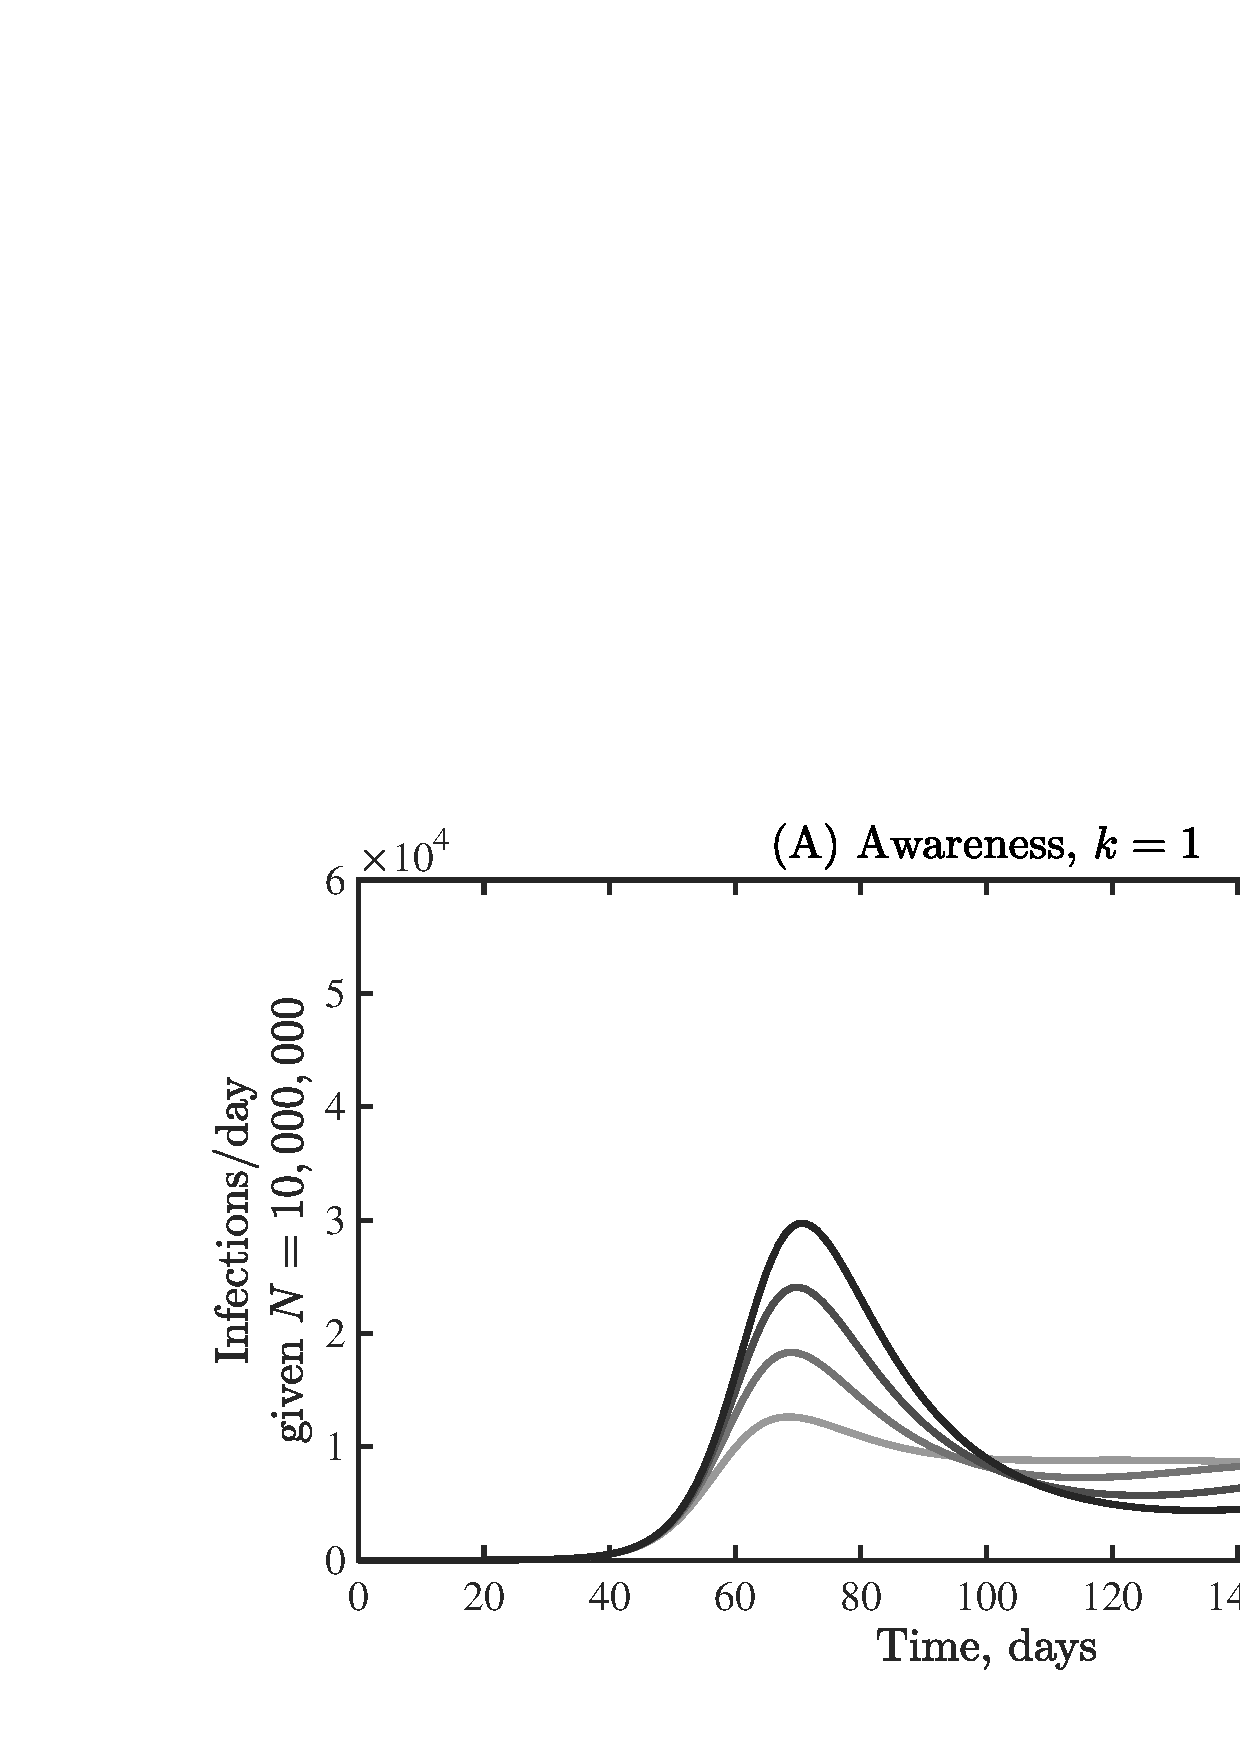
\includegraphics[width=0.45\textwidth]{figseir_Hdel_k1_noname.pdf}
%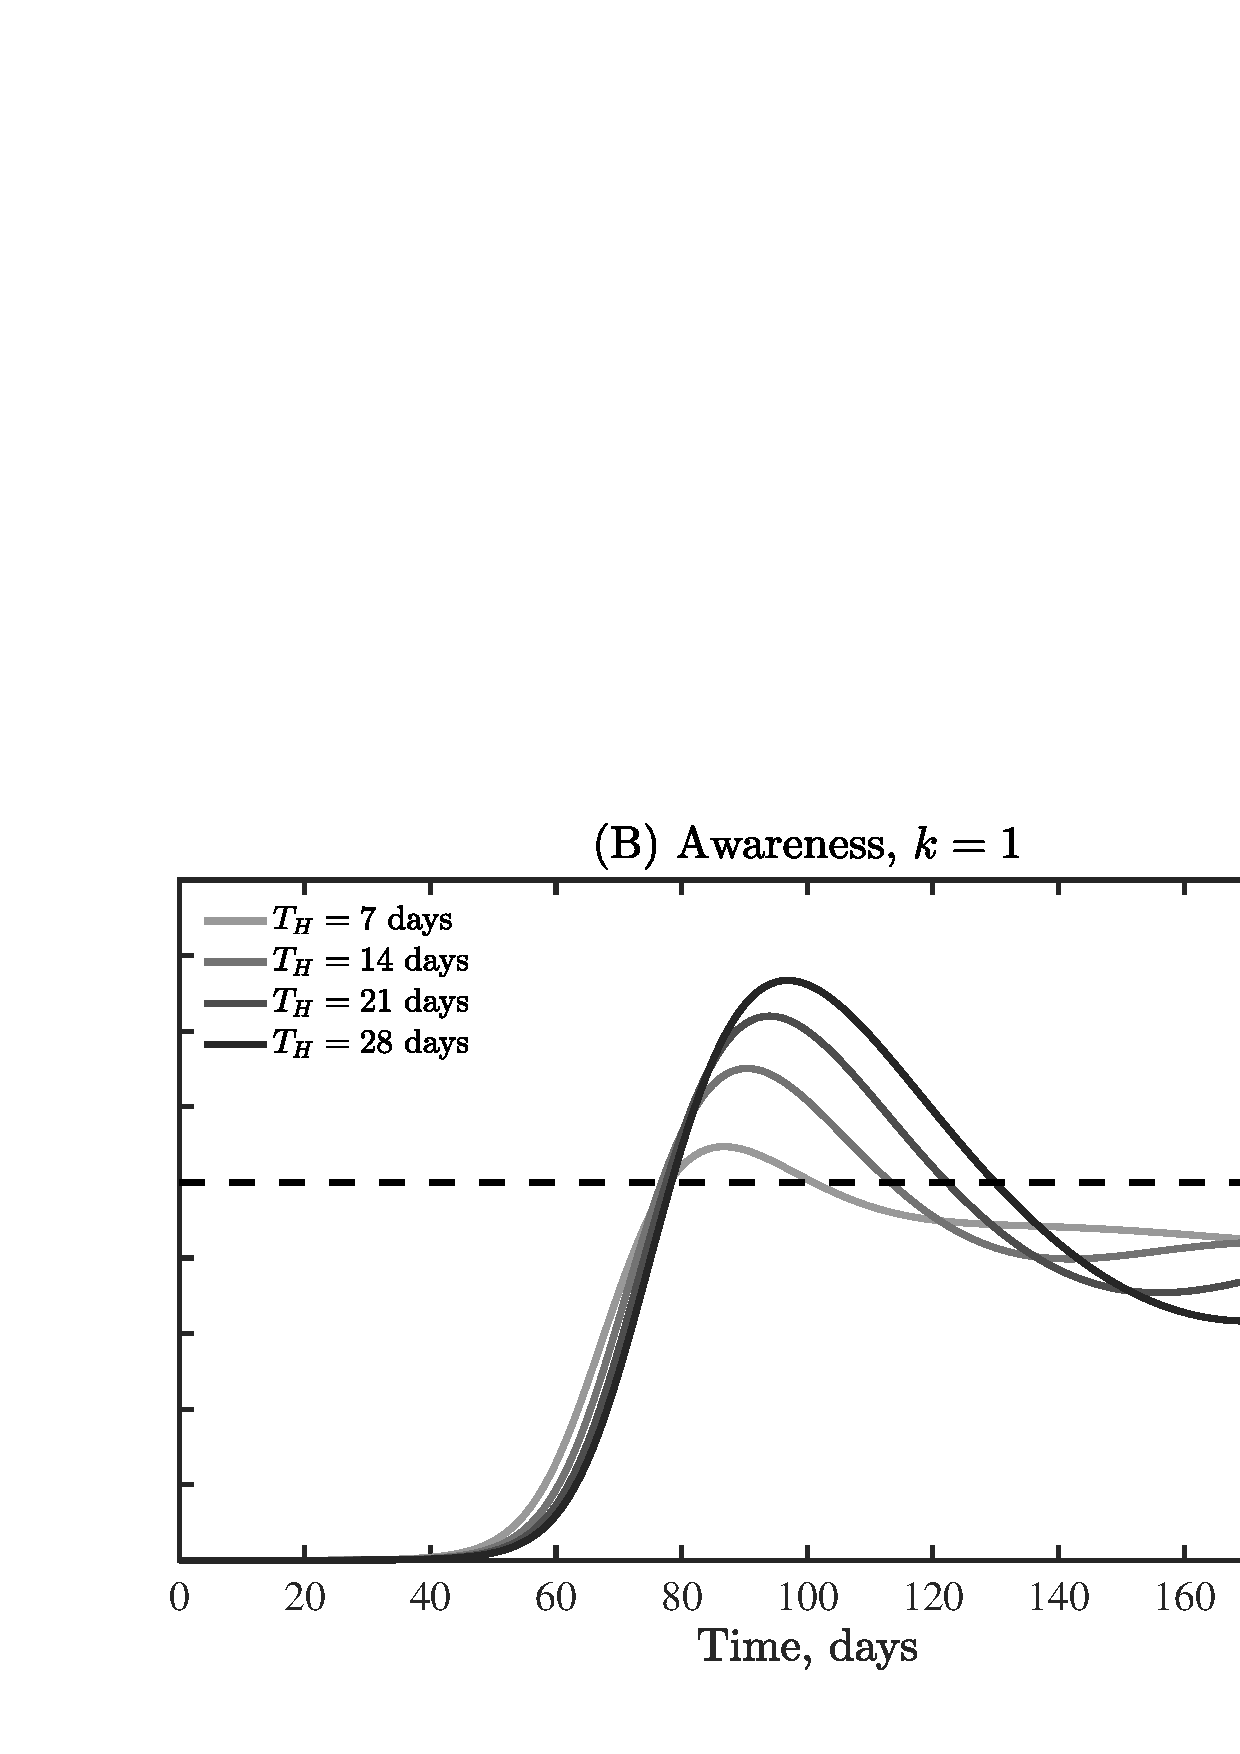
\includegraphics[width=0.45\textwidth]{figseir_Hdel_k1D_noname.pdf}\\
\includegraphics[width=0.485\textwidth]{scripts/figseir_Hdel_k2_noname.pdf}\\
\includegraphics[width=0.485\textwidth]{scripts/figseir_Hdel_k2D_noname.pdf}
%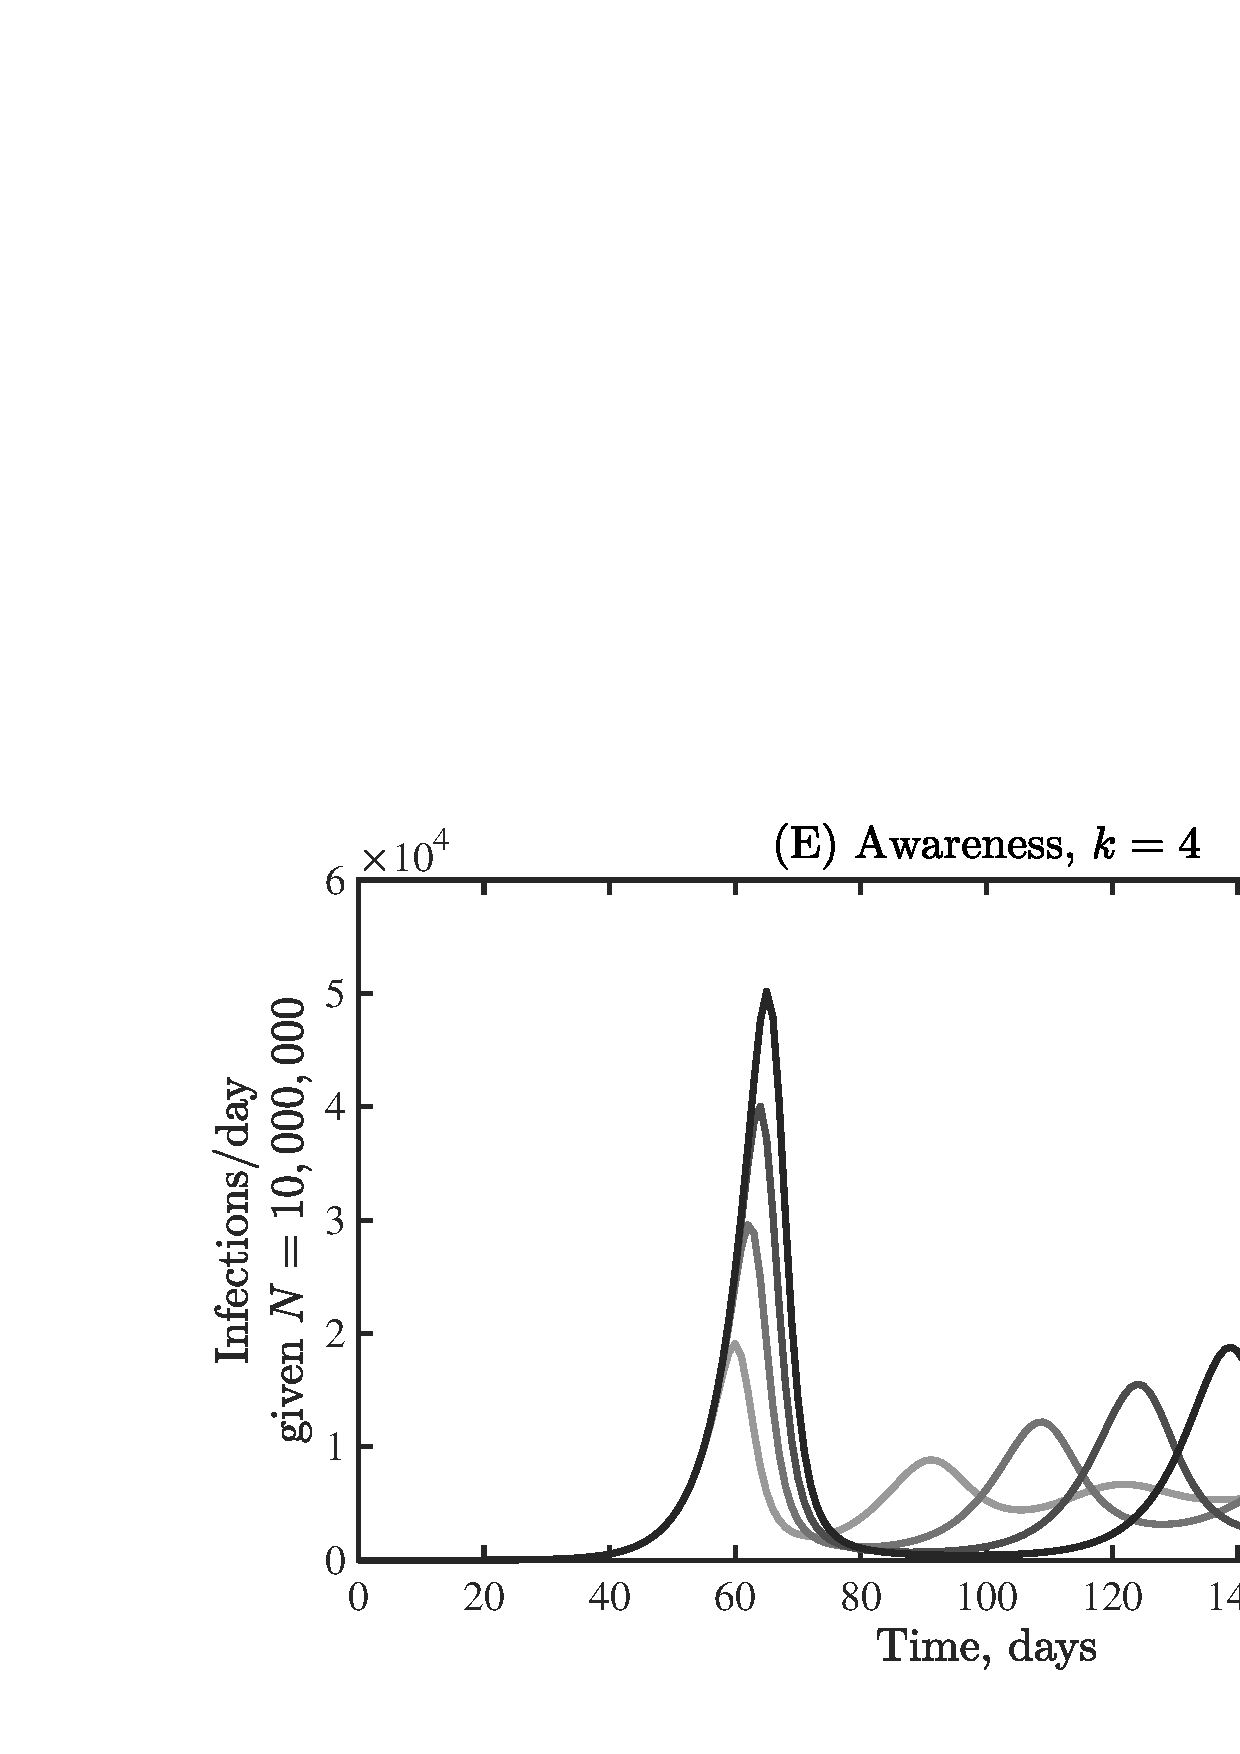
\includegraphics[width=0.45\textwidth]{figseir_Hdel_k4_noname.pdf}
%\includegraphics[width=0.45\textwidth]{figseir_Hdel_k4D_noname.pdf}\\
\caption{Emergence of oscillatory dynamics in a death-driven awareness
model of social distancing given lags between infection and fatality.
Awareness is $k=2$ and all other parameters as in Figure 2.
The dashed
lines for fatalities expected quasi-stationary value $\delta^{(q)}$.
\label{fig.oscillate}}
\end{center}
\end{figure}

\begin{figure}[t!]
\begin{center}
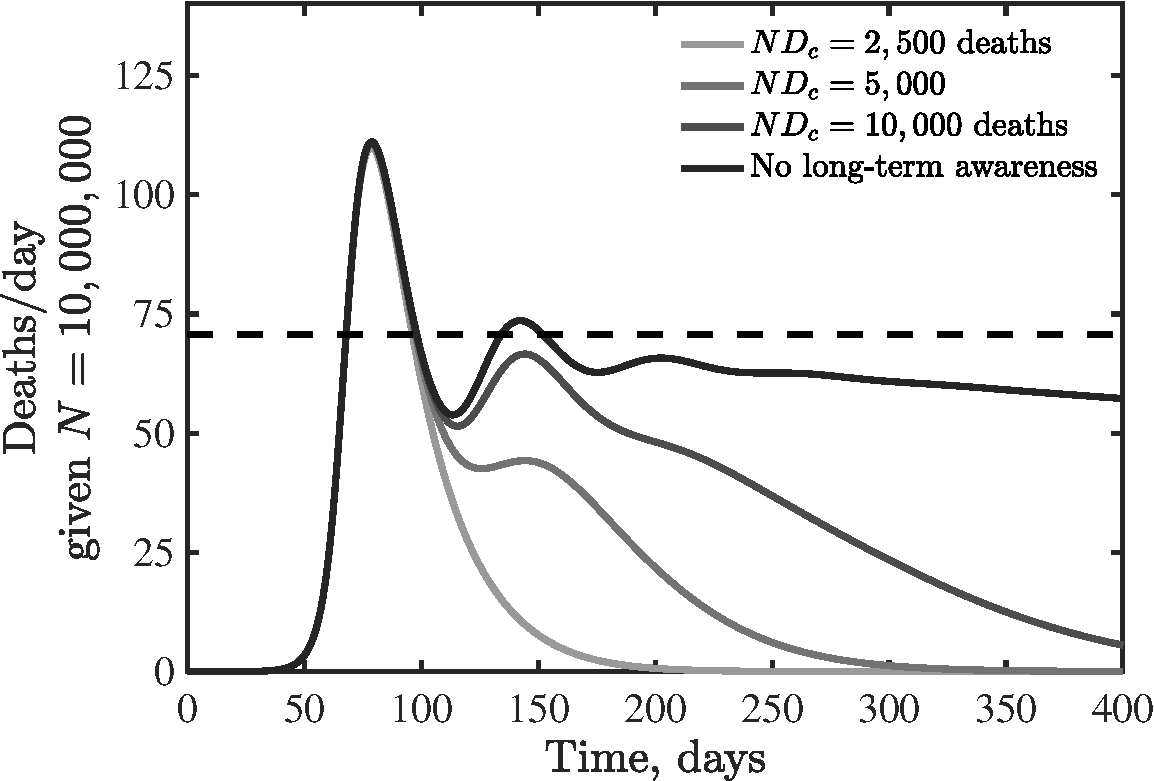
\includegraphics[width=0.47\textwidth]{scripts/figseir_Hlong_k2D_noname.pdf}\\
\includegraphics[width=0.47\textwidth]{scripts/figseir_Hlong_k2Dtot_noname.pdf}\\
\caption{SEIR dynamics with short- and long-term awareness.
Model parameters are $\beta=0.5$ /day, $\mu=1/2$ /day, $\gamma=1/6$ /day,
$T_H=14$ days, $f_D=0.01$, $N=10^7$, $k=2$, $N\delta_c=50$ /day (short-term
awareness), with varying $ND_c$ (long-term awareness) as shown in the legend.
The dashed line (top) denotes $\delta^{(q)}$ due to short-term
distancing alone.
\label{fig.longterm}}
\end{center}
\end{figure}

Finally, we recognize that awareness can vary in duration.  In previous
work, long-term awareness of cumulative incidence
was shown to lead to substantial decreases
in final size of epidemics compared
to baseline expectations from inferred 
strength~\citep{eksin2019systematic}. Hence, 
here we consider an extension of the SEIR model
with lags between infection and fatalities that incorporates
both short-term and long-term awareness:
\begin{eqnarray}
\dot{S} &=& -\frac{\beta SI}{\left[1+\left(\delta/\delta_c\right)^{k}+\left(D/D_c\right)^k\right]}\\
\dot{E} &=& \frac{\beta SI}{\left[1+\left(\delta/\delta_c\right)^{k}+\left(D/D_c\right)^k\right]}-\mu E\\
\dot{I} &=& \mu E-\gamma I \\
\dot{R} &=& (1-f_D)\gamma I\\
\dot{H} &=& f_D\gamma I - \gamma_H H\\
\dot{D} &=& \gamma_H H
\end{eqnarray}
where $D_c$ denotes a critical cumulative fatality level. 
Note that the relative importance of short- and long-term
awareness can be modulated by $\delta_c$ and $D_c$ respectively.
Figure~\ref{fig.longterm} shows cumulative fatalities (left)
and daily fatalities (right)
for a SEIR model with ${\cal{R}}_0=2.5$, $T_H=14$ days, and $N\delta_c=50$ 
fatalities per day and critical cumulative fatalities of
$ND_c=2,500$, 5,000, 10,000 as well as a comparison case with vanishing
long-term awareness. As is evident, 
long-term awareness drives dynamics towards rapid declines
after reaching a peak. This decline arises because
$D$ monotonically increases;
increasing fatalities beyond $D_c$ leads to rapid suppression
of transmission.  However, when $\delta_c$ rather than
$D_c$ drives dynamics, then shoulders and plateaus can re-emerge.
In reality, we expect that individual
behavior is shaped by short- and long-term awareness of risks, including
the potential for `decay' of long-term awareness~\citep{funk2009spread,funk2010modelling}.

In summary, we have shown how awareness of disease-induced death can reduce
transmission and also lead
to highly asymmetric epidemic curves, where the epidemic declines slowly 
even as the majority of the population remains susceptible.
In these conditions, if individuals are unable
to sustain social
distancing policies, or begin to tolerate higher death rates, then cases 
could increase. 
Hence: passing a `peak' need not imply
the rapid decline of risk.  These types of impacts of awareness-driven
endogenous changes in ${\cal{R}}_{\mathrm{eff}}$ are typically
absent in models that form the basis for public policy and strategic planning.
Moving forward, we hope that our findings
highlight the impacts of short-term and long-term awareness 
in efforts to shape information campaigns
to reduce transmission after early onset `peaks', particularly
when populations remain predominantly immunologically naive.
Although the models here are intentionally simple,
we contend that as cumulative data from COVID-19 outbreaks already
indicate, the asymmetric post-peak dynamics of COVID-19, including
slow declines and plateau-like behavior, may be an emergent
property of awareness-driven epidemiological dynamics.

